\subsection{[Aatos] NN analysis}

{\tt root\_v5.21.06}
Compiled with {\tt make -j2} option used for dual CPU machines.

\subsubsection{Default variables, default cuts}
\scriptsize
\begin{verbatim}
--- DataSet        : Prepare training and test samples:
--- DataSet        :     Signal tree     - number of events :  33972
--- DataSet        :     Background tree - number of events :  50259
--- DataSet        : Preselection:
--- DataSet        :     On signal input       : (((signalTracks == 1)&&(jetEt > 80))&&(abs(jeteta) < 2.4))
&&(ldgPt > 20)                                                                                            
--- DataSet        :     On background input   : (((signalTracks == 1)&&(jetEt > 80))&&(abs(jeteta) < 2.4))
&&(ldgPt > 20)                                                                                            
--- DataSet        :     Signal          - number of events :   4476    weighted :  4476
--- DataSet        :     Background      - number of events :   2627    weighted :  2627
--- DataSet        :     Signal          - efficiency       :                   0.131756
--- DataSet        :     Background      - efficiency       :                  0.0522692
--- DataSet        : Weight renormalisation mode: "NumEvents": renormalise signal and background
--- DataSet        :     weights independently so that Sum[i=1..N_j]{w_i} = N_j, j=signal, background
--- DataSet        :     (note that N_j is the sum of training and test events)
--- DataSet        : Event weights scaling factor:
--- DataSet        :     signal     : 1
--- DataSet        :     background : 1
--- DataSet        : Randomly pick events in training and testing trees for signal
--- DataSet        : Randomly pick events in training and testing trees for background
--- DataSet        : Create training tree
--- DataSet        : Create testing tree
--- DataSet        : Collected:
--- DataSet        : - Training signal entries     : 100
--- DataSet        : - Training background entries : 200
--- DataSet        : - Testing  signal entries     : 4376
--- DataSet        : - Testing  background entries : 2427
--- DataSet        : Compute correlation matrices on tree: TrainingTree
--- DataSet        : 
--- DataSet        : Correlation matrix (signal):
--- DataSet        : ------------------------------------------------------------------------------
--- DataSet        :                    jetEt  jeteta isolMaxPt50 ecalIsolEt10_50 hcalRatio    rtau
--- DataSet        :           jetEt:  +1.000  -0.172      -0.017          +0.122    +0.086  -0.029
--- DataSet        :          jeteta:  -0.172  +1.000      -0.073          -0.120    -0.141  -0.031
--- DataSet        :     isolMaxPt50:  -0.017  -0.073      +1.000          +0.126    +0.636  -0.491
--- DataSet        : ecalIsolEt10_50:  +0.122  -0.120      +0.126          +1.000    +0.045  -0.303
--- DataSet        :       hcalRatio:  +0.086  -0.141      +0.636          +0.045    +1.000  -0.615
--- DataSet        :            rtau:  -0.029  -0.031      -0.491          -0.303    -0.615  +1.000
--- DataSet        : ------------------------------------------------------------------------------
--- DataSet        : 
--- DataSet        : Correlation matrix (background):
--- DataSet        : ------------------------------------------------------------------------------
--- DataSet        :                    jetEt  jeteta isolMaxPt50 ecalIsolEt10_50 hcalRatio    rtau
--- DataSet        :           jetEt:  +1.000  +0.049      +0.283          +0.283    +0.106  -0.334
--- DataSet        :          jeteta:  +0.049  +1.000      -0.049          +0.031    +0.005  +0.037
--- DataSet        :     isolMaxPt50:  +0.283  -0.049      +1.000          +0.033    -0.063  -0.260
--- DataSet        : ecalIsolEt10_50:  +0.283  +0.031      +0.033          +1.000    -0.011  -0.179
--- DataSet        :       hcalRatio:  +0.106  +0.005      -0.063          -0.011    +1.000  -0.141
--- DataSet        :            rtau:  -0.334  +0.037      -0.260          -0.179    -0.141  +1.000
--- DataSet        : ------------------------------------------------------------------------------

--- NoTransform    : Ranking result (top variable is best ranked)
--- NoTransform    : ----------------------------------------------------------------
--- NoTransform    : Rank : Variable        : Separation
--- NoTransform    : ----------------------------------------------------------------
--- NoTransform    :    1 : isolMaxPt50     : 6.346e-01
--- NoTransform    :    2 : hcalRatio       : 5.483e-01
--- NoTransform    :    3 : rtau            : 4.809e-01
--- NoTransform    :    4 : ecalIsolEt10_50 : 2.657e-01
--- NoTransform    :    5 : jeteta          : 2.596e-01
--- NoTransform    :    6 : jetEt           : 1.679e-01
--- NoTransform    : ----------------------------------------------------------------

MLP  H:!V:!Normalise:NeuronType=tanh:NCycles=1000:HiddenLayers=N+5:TestRate=5

--- MLP            : ----------------------------------------------------------------
--- MLP            : Rank : Variable        : Importance
--- MLP            : ----------------------------------------------------------------
--- MLP            :    1 : rtau            : 2.999e+00
--- MLP            :    2 : jeteta          : 2.042e+00
--- MLP            :    3 : jetEt           : 1.706e+00
--- MLP            :    4 : isolMaxPt50     : 4.264e-03
--- MLP            :    5 : ecalIsolEt10_50 : 1.268e-03
--- MLP            :    6 : hcalRatio       : 3.935e-06
--- MLP            : ----------------------------------------------------------------

--- Factory        : Evaluation results ranked by best signal efficiency and purity (area)
--- Factory        : -----------------------------------------------------------------------------
--- Factory        : MVA              Signal efficiency at bkg eff. (error):  |  Sepa-    Signifi-
--- Factory        : Methods:         @B=0.01    @B=0.10    @B=0.30    Area   |  ration:  cance:  
--- Factory        : -----------------------------------------------------------------------------
--- Factory        : MLP            : 0.586(07)  0.812(05)  0.888(04)  0.906  |  0.576    1.508
--- Factory        : -----------------------------------------------------------------------------
--- Factory        : 
--- Factory        : Testing efficiency compared to training efficiency (overtraining check)
--- Factory        : -----------------------------------------------------------------------------
--- Factory        : MVA           Signal efficiency: from test sample (from traing sample) 
--- Factory        : Methods:         @B=0.01             @B=0.10            @B=0.30   
--- Factory        : -----------------------------------------------------------------------------
--- Factory        : MLP            : 0.586 (0.325)       0.812 (0.833)      0.888 (0.898)
--- Factory        : -----------------------------------------------------------------------------


--- ==================================================================================================
--- Classifier   (  #signal, #backgr.)  Optimal-cut  S/sqrt(S+B)      NSig      NBkg   EffSig   EffBkg
--- --------------------------------------------------------------------------------------------------
---        MLP:  (     1000,     1000)      -0.2355      26.9054  803.0164  87.76267    0.803  0.08776
--- --------------------------------------------------------------------------------------------------

--- Factory        : Evaluating all classifiers for signal efficiency @ 1e-5 OVERALL bkg efficiency
--- Factory        : 
--- Factory        :                                   signal   background
--- Factory        : Event preselection efficiency   : 1.00000  1.00000
--- Factory        : Jet preselection efficiency     : 0.13176  0.05227
--- Factory        : -----------------------------------------------------
--- Factory        : Overall preselection efficiency : 0.13176  0.05227
--- Factory        : 
--- Factory        : Thus the 1e-5 overall bkg efficiency corresponds 1.913171e-04 bkg efficiency in TMVA
--- Factory        : 
--- Factory        : Evaluation results ranked by best signal efficiency
--- Factory        : -----------------------------------------------------------------------------
--- Factory        : MVA              Signal efficiency at 1e-5 overall bkg eff.:
--- Factory        : Methods:         TMVA       with preselection
--- Factory        : -----------------------------------------------------------------------------
--- Factory        : MLP_v0         : 0.04700     0.00619
--- Factory        : MLP_v1         : 0.00025     0.00003

\end{verbatim}
\normalsize

(See Figs.\ref{fig:variables_c1},
 
\begin{figure}[h]
\begin{center}
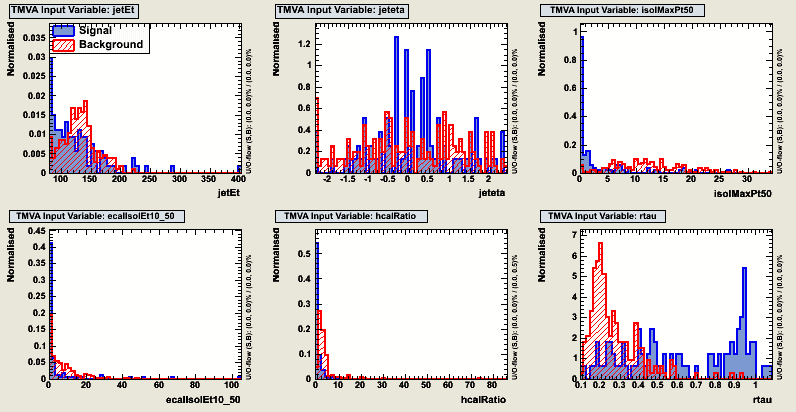
\includegraphics[width=1.0\textwidth]{images/ahVariables_c1.png}
\caption{Variables used in the analysis. Notice log transformations used for some of the variables.}
\label{fig:variables_c1}
\end{center}
\end{figure}

\begin{figure}[h]
\begin{center}
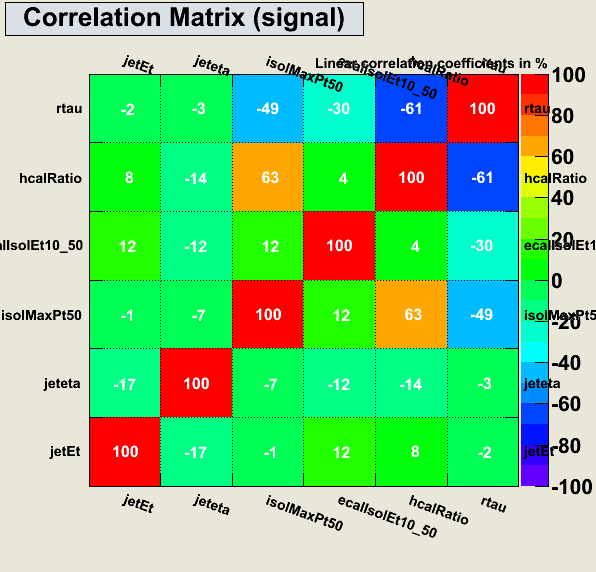
\includegraphics[width=0.5\textwidth]{images/ahCorrelationMatrixS.png}
\caption{Variable correlation matrix for signal}
\label{fig:ahCorrelationMatrixS}
\end{center}
\end{figure}

\begin{figure}[h]

\begin{center}
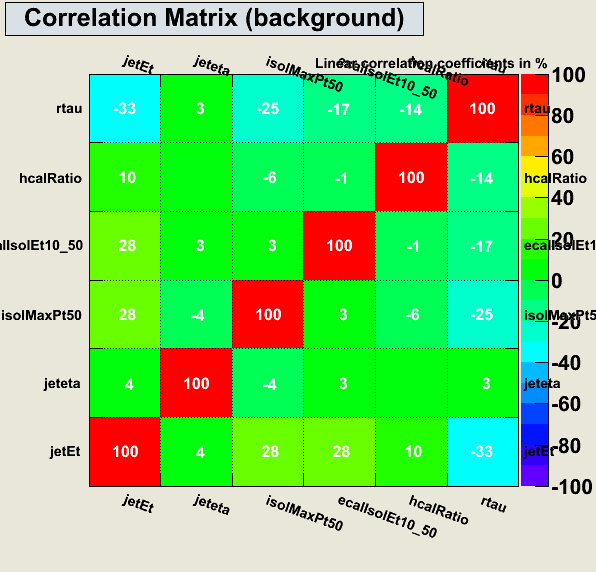
\includegraphics[width=0.5\textwidth]{images/ahCorrelationMatrixB.png}
\caption{Variable correlation matrix for background}
\label{fig:ahCorrelationMatrixB}
\end{center}
\end{figure}

\begin{figure}[h]
\begin{center}
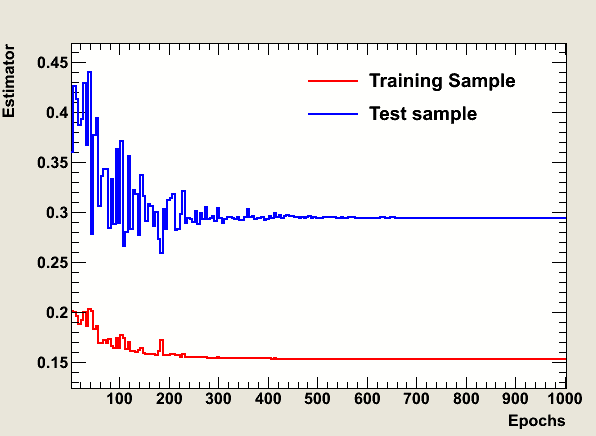
\includegraphics[width=1.0\textwidth]{images/ahAnnconvergencetest.png}
\caption{ANN convergence test}
\label{fig:ahAnnconvergencetest}
\end{center}
\end{figure}




\begin{figure}[h]
\begin{center}
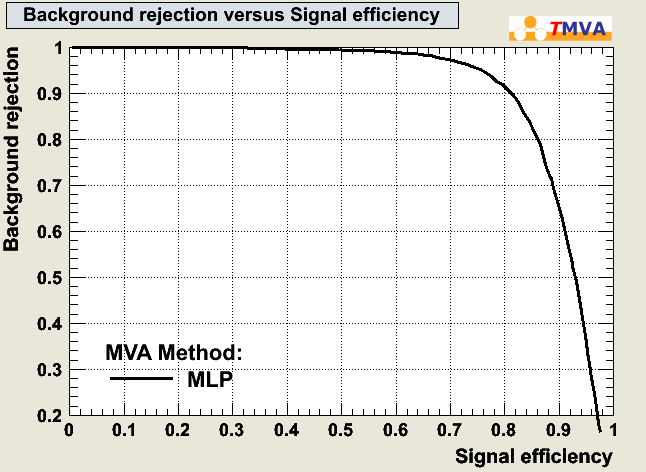
\includegraphics[width=1.0\textwidth]{images/ahRejBvsS.png}
\caption{Rejection B vs. S}
\label{fig:ahRejBvsS}
\end{center}
\end{figure}



\begin{figure}[h]
\begin{center}
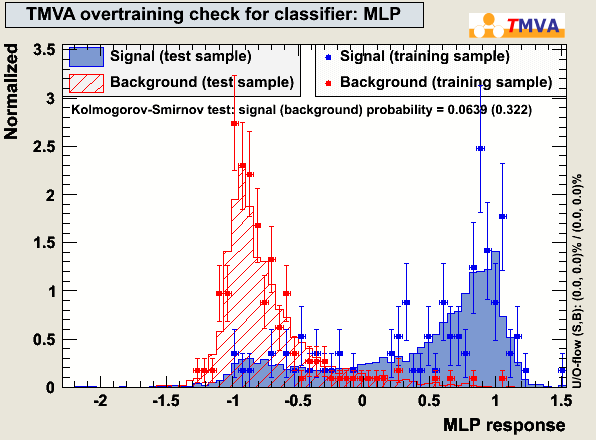
\includegraphics[width=1.0\textwidth]{images/ahOvertrain_MLP.png}
\caption{Overtrain?}
\label{fig:overtrainmlp}
\end{center}
\end{figure}

\clearpage

\begin{figure}[!h]
\begin{center}
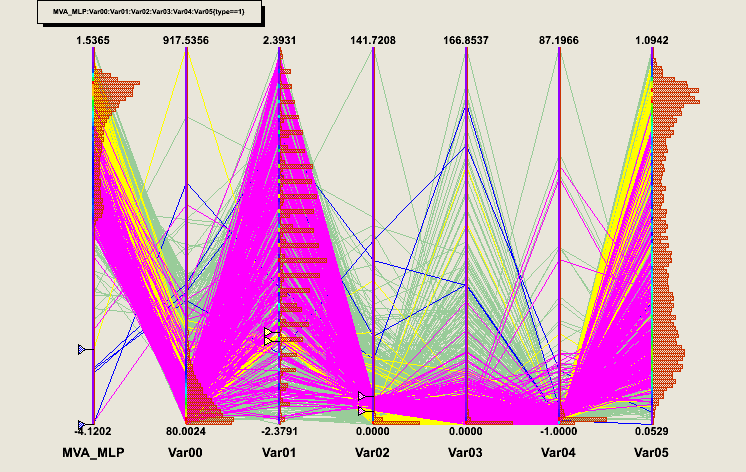
\includegraphics[width=0.8\textwidth]{images/ahParacoor_c0_S.png}
\caption{Parallel coordinates for signal. 
(For more information on parallel coordinates plot see \url{http://en.wikipedia.org/wiki/Parallel_coordinates}.)}
\label{fig:ahParacoor_c0_S}
\end{center}
\end{figure}
\begin{figure}[!h]
\begin{center}
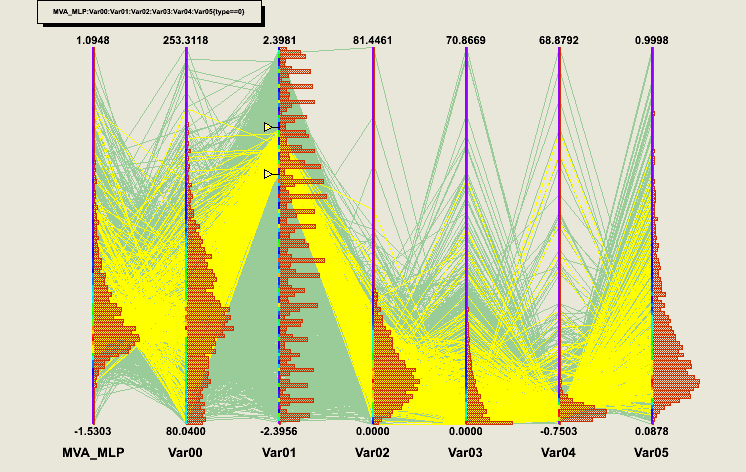
\includegraphics[width=0.8\textwidth]{images/ahParacoor_c0_B.png}
\caption{Parallel coordinates for background}
\label{fig:ahParacoor_c0_B}
\end{center}
\end{figure}

\clearpage

\begin{figure}[h]
\begin{center}
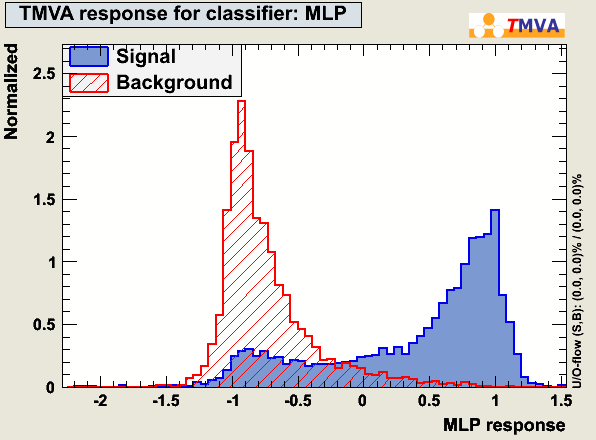
\includegraphics[width=1.0\textwidth]{images/ahMva_MLP.png}
\caption{mva MLP}
\label{fig:mvamlp}
\end{center}
\end{figure}


\subsection{tmva-common.conf}
\lstset{
language=bash,
numbers=left,
stepnumber=2,
caption={\tt code/tmva-aatos.conf},
label=tmvacommonconf
}
\lstinputlisting{code/tmva-aatos.conf}

%git fetch pekka
%git merge pekka/master
%gitk 
%(modify)
%git diff
%git status
%git commit -a -m 'comment'  (add all changes)
%(modify)
%git diff
%git commit -a -m 'comment'  

%gitk 
%git revert HEAD  (in case of bad commit this reverses it)

%git push 

%make release


%.gitconfig}:
%
%[user]
%	email = aatos.heikkinen@cern.ch
%[color]
%       ui = auto






